\documentclass[hyperref={pdfpagelabels=true}]{beamer}

\usepackage{lmodern}
%%%%%%%%%%%%%%%%%%%%%%%%%%%%%%%%%%%%%%%%%%%%%%%%%%%%%%%%%%%%%%%%%%%%%%%%%%%%%%%%%%%%%%%%%%%%%%%%%
%This work is licensed under a Creative Commons Attribution-ShareAlike 4.0 International License.
%
%You are free to:
%
%    Share — copy and redistribute the material in any medium or format
%    Adapt — remix, transform, and build upon the material
%    for any purpose, even commercially.
%
%    The licensor cannot revoke these freedoms as long as you follow the license terms.
%
%Attribution — You must give appropriate credit, provide a link to the license, and indicate if changes were made. You may do so in any reasonable manner, but not in any way that suggests the licensor endorses you or your use.
%
%ShareAlike — If you remix, transform, or build upon the material, you must distribute your contributions under the same license as the original. 
%
%%%%%%%%%%%%%%%%%%%%%%%%%%%%%%%%%%%%%%%%%%%%%%%%%%%%%%%%%%%%%%%%%%%%%%%%%%%%%%%%%%%%%%%%%%%%%%%%%
\definecolor{dred}{rgb}{0.647059, 0.164706, 0.164706}
\definecolor{dgreen}{rgb}{0., 0.545098, 0.545098}
\usecolortheme[named=dred]{structure}

\title{Crunching and visualizing Big Data}
\subtitle{on a Computer Cluster}
\author{Joana Sim\~{o}es} 

%\author[shortname]{Joana Sim\~{o}es \inst{1}}
%\institute[shortinst]{\inst{1} Bdigital, CASA, CICS.NOVA}

%\date{\today} 
%\titlegraphic{\includegraphics[width=.35\textwidth]{bigdata2.png}}
 
\usepackage{beamerthemeshadow}
%\usepackage{beamerthemesplit}
\usepackage{listings}

\newcommand{\soooo}{H$_2$SO$_4$}

%fdl stuff
\usepackage{hyperref}
\hypersetup{colorlinks, 
           citecolor=black,
           filecolor=black,
           linkcolor=black,
           urlcolor=black,
           bookmarksopen=true,
           pdftex}

\hfuzz = .6pt % avoid black boxes

\lstset{language=SQL}

\begin{document}
\setbeamertemplate{footline}[page number]
\setbeamertemplate{navigation symbols}{}
\begin{frame}
%\titlepage

\begin{titlepage}
\centering{ 
  
\includegraphics[height=50px]{hadoop.png}    
  
\includegraphics[height=50px]{esri.jpg}  
  
\includegraphics[height=50px]{pig.png}    
  
\includegraphics[height=50px]{postgis.png}    
  
\includegraphics[height=50px]{es.jpeg}  
  
\includegraphics[height=50px]{kibana.png}  
}
\end{titlepage}

\end{frame} 
  
 
\begin{frame}
\frametitle{Table of Contents}
%\tiny{
\tableofcontents%}
\end{frame}

\section{Introduction} 
%marcs stack
% machine learning/data mining, processing data
%There are no freelunches

%todo: introduce the dataset, introduce the tools; 
%start and connect to the cluster
%  \item<1->It can be run in interactive mode, or in batch mode

\section{Importing a Spatial-Temporal Series} 

\begin{frame}
\frametitle{From S3 to HDFS}
\begin{itemize}
  \item<1->Micro-task: Understand the dataset structure
  \begin{itemize}
    \item<1->A sample dataset is stored on an S3 bucket: \url{s3n://workshop-bdsd/accidents/}
    \item<2->\textbf{\url{https://s3-eu-west-1.amazonaws.com/workshop-bdsd/accidents/accidents\_sample.csv}}
    \item<3->Download and view dataset
  \end{itemize}
\end{itemize}
\end{frame}

\begin{frame}
\frametitle{From S3 to HDFS (cont.)}
\begin{itemize}
  \item<1->Micro-task: Create a table linking to the data
  \begin{itemize}
    \item<1->Enter hive and create an external table linking to the S3 bucket
    \item<2->Use the CSV serde to parse the table structure
      \begin{itemize}
	\item<3->separator char
	\item<3->quote char
	\item<3->headers
       \end{itemize}
    \item<4->View imported data       
  \end{itemize}
\end{itemize}
\end{frame}

\begin{frame}
\frametitle{From S3 to HDFS (cont.)}
\begin{itemize}
  \item<1->Micro-task: Type Mapping
  \begin{itemize}
    \item<2->Create an empty table with correct types
    \item<3->Insert data from accidents\_import
    \item<4->View table
  \end{itemize}
\end{itemize}
\end{frame}

\section{Recovering the Spatial Attributes} 

\begin{frame}
\frametitle{What is so "Special" about Spatial}
\begin{columns}
  \begin{column}{0.5\textwidth}
    \begin{itemize}
      \item<2-> Location attributes allow us to detect spatial patterns
      \item<2-> Location also works as a "key", allowing us to connect with other datasets
    \end{itemize}    
  \end{column}
  
  \begin{column}{0.5\textwidth}
      \begin{figure}  
	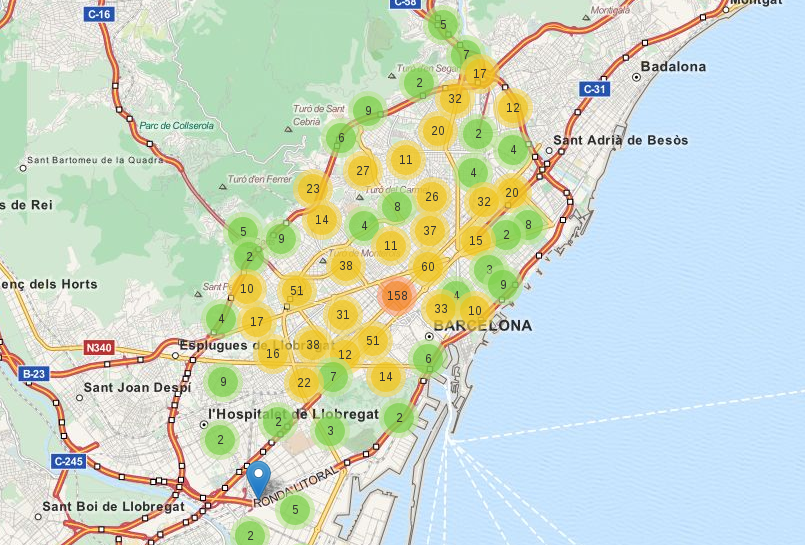
\includegraphics[width=\textwidth]{bettermap.png}\\
       \end{figure}  
  \end{column}  
\end{columns}
\end{frame}

\begin{frame}
\frametitle{Analysis of the Spatial Attributes}
    \begin{itemize}
      \item<1-> Spatial Attributes are encoded as coordinates in "d\_coord\_geo\_impacte"
      \item<2-> Problems with this field:
      \begin{itemize}
	\item<3->Unstructured: needs parsing
	\item<3->Inconsistent format (order of coordinates, separator)	
	\item<3->Invalid values (e.g.: 77, names)
	\item<3->No metadata	
	\item<4->Mixed CRS:
	  \begin{itemize}
	  \item<5->WGS84 (EPSG:4326)
	  \item<5->UTM Grid (EPSG:5554)
	  \item<5->UTM Grid encoded by the police using an \textit{ad-hoc} format
%	    \begin{itemize}
	    \item<6->$lon = y/ 1000 + 400000$
	    \item<6->$lat = y/ 1000 + 4500000$	    
	    \end{itemize}        		  
%	  \end{itemize}        	
      \end{itemize}        
    \end{itemize}    
\end{frame}

%TODO: SLIDE WITH COORDS

\begin{frame}
\frametitle{Objective}
\begin{itemize}
  \item<1->Separate lat, long fields and map them to correct types
  \item<1->Remove invalid values  
  \item<1->Convert all coordinates into a single CRS (WGS84)
\end{itemize}
\end{frame}

\begin{frame}
\frametitle{Exporting Data to Pig}
\begin{itemize}
  \item<1->Pig uses filters to subset the data
  \item<1->To merge back the subsetted data, we can use joins by a common field  
  \item<1->Micro-task: Export the data
  \begin{itemize}
    \item<2->Create a copy of the accidents table, with an id field (joins).
    \item<3->Export this table into a tsv
    \item<4->Store it in HDFS (if needed)
    \item<4->View exported data    
  \end{itemize}
\end{itemize}
\end{frame}

\begin{frame}
\frametitle{Presenting the Pig Script}
\begin{columns}
  \begin{column}{0.5\textwidth}
    \begin{itemize}
      \item<1->Subsets the coordinate list, using filters
      \item<1->Detects each coordinate "type", using regular expressions
      \item<1->In the case of UTM encoded, it applies a formula to decode back into UTM
      \item<1->Stores the results into separate files, in HDFS  
    \end{itemize}
  \end{column}  
  \begin{column}{0.5\textwidth}
      \begin{figure}  
	
\includegraphics[width=\textwidth]{pig-on-elephant.png}
       \end{figure}  
  \end{column}  
\end{columns}
\end{frame}

\begin{frame}
\frametitle{REGEX}
\begin{columns}
  \begin{column}{0.5\textwidth}
    \begin{itemize}
      \item<1->Sequence of characters that forms a search pattern, mainly for use in pattern matching with strings, or string matching%find and replace
      \item<2->REGEX\_EXTRACT(D\_COORD\_GEO\_IMPACTE,'[A-z]',0)
      \item<3->'[A-z]'%any character, upper case and lower case  
    \end{itemize}
  \end{column}  
  \begin{column}{0.5\textwidth}
      \begin{figure}  
	
\includegraphics[width=\textwidth]{yesterdays-regex.jpg}\\	
       \end{figure}  
        %\tiny{Read more: \url{http://www.regular-expressions.info/}}           
  \end{column}  
\end{columns}        
\end{frame}

\begin{frame}
\frametitle{Running Pig}
\begin{itemize}
  \item<1->Micro-task: run pig script
  \begin{itemize}
    \item<2->Download script from S3: \url{https://s3-eu-west-1.amazonaws.com/workshop-bdsd/recover_geography.pig}
    \item<3->Edit script and \textbf{ammend paths}
    \item<4->Run script    
    \item<5->Check output files
  \end{itemize}
\end{itemize}
\end{frame}

\begin{frame}
\frametitle{Importing Data Back into Hive}
\begin{itemize}
  \item<1->Micro-task: Create tables linking to pig output
  \begin{itemize}
    \item<2->Create table with wgs84 data
    \item<2->Create table with UTM data
    \item<2->Create table with police-decoded data
  \end{itemize}
\end{itemize}
\end{frame}

\begin{frame}
\frametitle{Exporting data into PostGIS}
\begin{columns}
  \begin{column}{0.5\textwidth}
    \begin{itemize}
      \item<1->As of Hadoop GIS 2.0, CRS transformation is \textbf{not supported}
      \item<1->We need to rely on another tool: PostGIS on RDS  
      \item<1->Micro-task: Export UTM data to PostGIS
      \begin{itemize}
	\item<2->Merge UTM (UTM + police) tables in a single table
	\item<3->Exported merged table into TSV
      \end{itemize}
    \end{itemize}
  \end{column}  
  \begin{column}{0.5\textwidth}
      \begin{figure}  
	
\includegraphics[width=0.8\textwidth]{postgis.png}	
       \end{figure}  
  \end{column}  
\end{columns}        
\end{frame}


\begin{frame}
\frametitle{Importing Data into PostGIS}
\begin{itemize}
  \item<1->Micro-task: Import UTM data into PostGIS
  \begin{itemize}
    \item<2->Install the PSQL client
    \item<2->Log into RDS:
    \begin{itemize}    
      \item<3->host: bdigitaldb.celqzuwfokoe.eu-west-1.rds.amazonaws.com
      \item<3->user: workshop
      \item<3->password: geohipster
      \item<3->database: workshop\_bdigital      
    \end{itemize}
    \item<4->Create table to accomodate data
    \item<5->Copy data into table
    %\item<6->Create geometric fields to accomodate geometry in the two CRS (WGS,UTM)
  \end{itemize}
\end{itemize}
\end{frame}

\begin{frame}
\frametitle{CRS Transformation}
\begin{itemize}
  \item<1->Micro-task: Convert all features in UTM grid to WGS84
  \begin{itemize}
    \item<2->Create geometry fields to accomodate geometry in the two CRS (UTM, WGS84)
    \begin{itemize}    
      \item<3->Add columns
      \item<3->Set SRID
      \item<3->Create geometry index
    \end{itemize}
    \item<4->Instantiate UTM geometry
    \item<5->Transform UTM geometry into another CRS
    \item<6->Export projected geometry in GeoJSON
  \end{itemize}
\end{itemize}
\end{frame}

%TODO: GeoJSON

\begin{frame}
\frametitle{Importing Data back into Hive}
\begin{itemize}
  \item<1->Micro-task: Import transformed data
  \begin{itemize}
    \item<2->Enter Hive
    \item<3->Create table linking to the PostGIS export    
    \item<4->Create new table and instantiate geometry from GeoJSON
  \end{itemize}
\end{itemize}
\end{frame}

%\section{Recovering the Timestamps} 

\section{Putting it All Together} 
%final queries
\begin{frame}
\frametitle{Joining Data}
\begin{itemize}
  \item<1->Micro-task: Join imported coordinates with WGS84 coordinates and the rest of the dataset
  \begin{itemize}
    \item<2->Join imported records with original table with all fields
    \item<3->Merge imported records with WGS84 records, for a single table with unified geometry
  \end{itemize}
\end{itemize}
\end{frame}

\section{Piping the Results into the Outside World} 
%introduce ES
%export data to ES

\begin{frame}
\frametitle{References}
\begin{itemize}\tiny{
\item \url{http://tweettracker.fulton.asu.edu/tda/TwitterDataAnalytics.pdf}
\item \url{http://www2.qgis.org}
\item \url{http://plugins.qgis.org/plugins/}
\item \url{http://geokoder.com/mongodb-plugin-for-quantum-gis}
\item \url{http://www.gislounge.com/heat-maps-in-gis/}
\item \url{https://alastaira.wordpress.com/2011/02/23/heat-mapping-crime-data-with-bing-maps-and-html5-canvas/}
\item \url{http://docs.qgis.org/2.0/en/docs/user_manual/plugins/plugins_heatmap.html}
\item \url{http://en.wikipedia.org/wiki/Kernel_\%28statistics\%29\#Kernel\_functions\_in\_common\_use}
\item \url{http://en.wikipedia.org/wiki/Cluster_analysis}
\item \url{https://plugins.qgis.org/plugins/clusterpy_qgis_plugin/}
\item \url{http://www.rise-group.org/section/Software/clusterPy/}
\item \url{http://threejs.org/}
\item \url{http://anitagraser.com/2014/03/15/3d-viz-with-qgis-three-js/} }
\end{itemize}
\end{frame}

\begin{frame}
\frametitle{Thank you for Listening!}
    \begin{figure}  
      
\includegraphics[width=0.8\textwidth]{fat-cat.jpg}    
     \end{figure}  
\end{frame}


\end{document}